\begin{figure}[ht!]
    \centering
    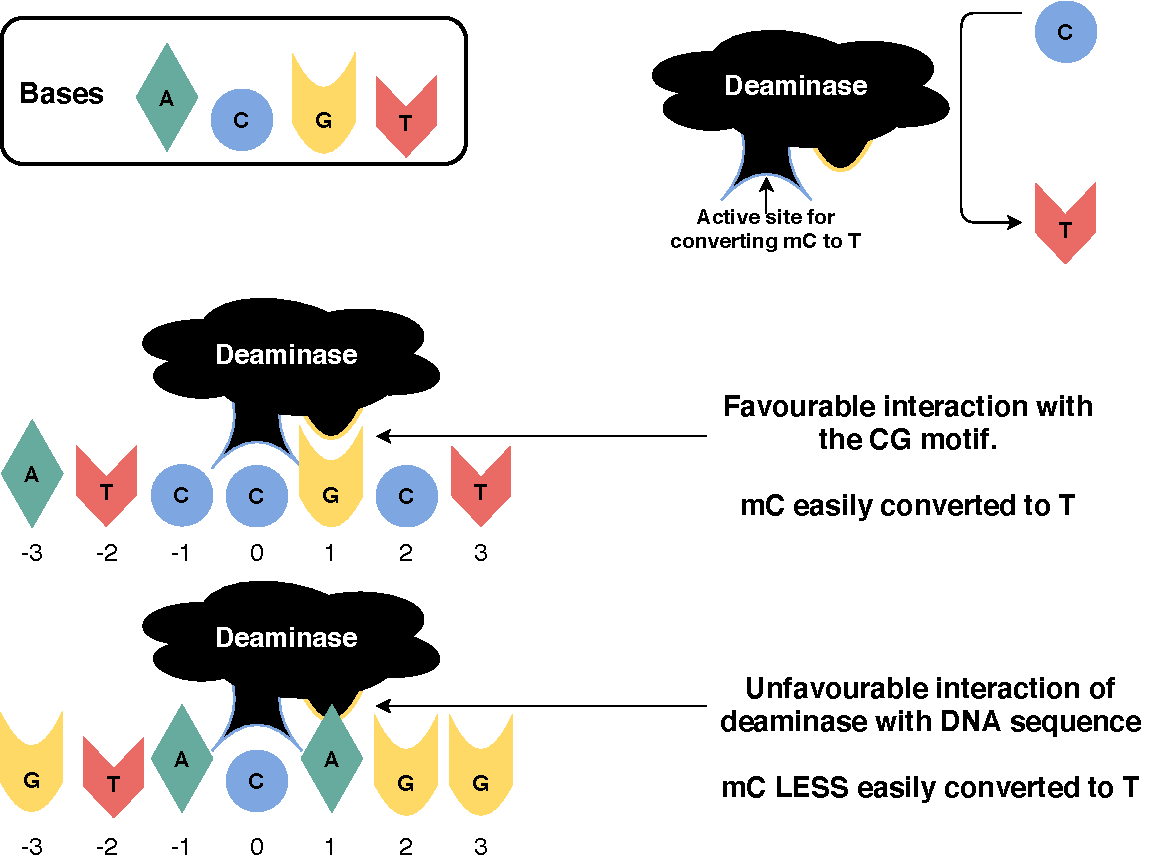
\includegraphics[scale=0.75]{graphics/motif_demo.pdf}
    \caption{\textbf{Methyltransferase activity as an example to explain how mutations are closely linked with the bases next to them}. Methyltransferase favours the CpG motif, so the cytosine (C) in CpG is easily methylated into methyl-cytosine in mCpG. mC is an ``excited'' state that is prone to C$\rightarrow$T mutations. Base abbreviations: A=Adenine, C=Cytosine, G=Guanine, T=Thymine.}
    \label{fig:motif_demo}
\end{figure}
